\section{D mesons efficiencies}
\label{sec:eff}
The prompt D meson production yields were calculated by correcting the measured inclusive raw yields, $N^{raw}$, for the B meson decay feed-down contribution and dividing by the acceptance times efficiency for prompt D mesons,(Acc$\times \epsilon$)$_{prompt}$.  They were normalised according to the decay channel branching ratio (BR), \pt interval width ($\Delta$\pt), rapidity coverage ($\Delta y$), and the number of events analysed ($N_{\mathrm{evt}}$). 
They were then divided by a factor of two to evaluate the charge (particle and anti-particle) averaged yields. As an illustration, the \Dzero yields were computed as:
\begin{equation}
 \label{eq:effMethod}
 \frac{\mathrm{d}N}{\mathrm{d}p_{\mathrm{T}}}\bigg\rvert_{|y|<0.5} = \frac{1}{2}\frac{1}{\Delta p_{\mathrm{T}}} \frac{f_{\mathrm{prompt}}(p_{\mathrm{T}})\cdot N^{\mathrm{D^{0}raw}}(p_{\mathrm{T}})\bigg\rvert_{|y| < y_{\mathrm{fid}}}}{(\mathrm{Acc}\times\epsilon)_{\mathrm{prompt}}(p_{\mathrm{T}})\cdot \mathrm{BR} \cdot N_{\mathrm{evt}} }
\end{equation}

Where $f_{\mathrm{prompt}}$ is the prompt D meson fraction in a given \pt bin. The D meson yields were measured in a rapidity range varying from $|y|<$ 0.5 at low \pt to $|y|<$ 0.8 at high \pt. The rapidity acceptance correction factor $\Delta y$=2$y_{\mathrm{fid}}$ assumes a uniform rapidity distribution for D mesons in the measured $y$ range. This assumption was verified to the 1$\%$ level with PYTHIA \cite{Sjostrand:2006za} proton--proton simulations with the Perugia-0 \cite{Skands:2009zm} tuning.
The acceptance times efficiency corrections Acc$\times \epsilon$ were obtained using Monte Carlo simulations. \pbpb collisions at \sNN 5.02 TeV were produced with the HIJING v1.36 \cite{Wang:1991hta} event generator. Prompt and feed-down (B decays) D meson signals were added using \pp events from the PYTHIA v6.4.21 event generator with the Perugia-0 tuning.  Each injected \pp event was required to contain a c$\overline{\mathrm{c}}$ or b$\overline{\mathrm{b}}$ pair and D mesons were forced to decay in the hadronic channels of interest for the analysis.  Only particle coming from the heavy quark hadronization and decays were injected in the HIJING event.  The number of \pp events added to each \pbpb event was adjusted according to the \pbpb collision centrality. 
The simulations used the GEANT3 particle transport package together with a detailed description of the geometry of the apparatus and of the detector response. The simulation was configured to reproduce the conditions of the luminous region and of all the ALICE subsystems, in terms of active electronic channels, calibration level, and their time evolution within the \pbpb data taking period.

The impact parameter distribution in LHC18q and LHC18r has been studied in detail. For these two data taking periods the impact parameter distributions have been investigated as a function of \pt and in 24 $\phi$ bins, in order to apply more precise corrections to the impact parameter distributions in the MC productions.
The impact parameter distribution is shifted by up to $\pm$20-30 micron at low \pt and to $\pm$5-10 micron at high \pt. The shift depends on the azimuthal angle and this is not described in the MC. Current hypothesis is that part of the shift is due to the presence of SPD modules that were not included in the latest re-alignment (because they were included only recently in the data taking). The impact parameter resolution measured in data were reproduced in MC using the task \texttt{PWGHF/vertexingHF/AliAnalysisTaskSEImproveITS.cxx}. The task has been used with the option \texttt{SetMimicData(kTRUE)}, which scales in the MC the residuals $d_0$(true)-$d_0$(reco) according to the ratio data/MC of the impact parameter resolutions (for more details see...)

The efficiencies were evaluated in a centrality class corresponding to the one used in the analysis of the data in terms of charged particle multiplicity,  hence of the detector occupancy. Figure \ref{fig:Dzero_eff_acc} shows the \Dzero$\rightarrow$ K$^{-}\pi^{+}$ efficiency $\times$ acceptance for prompt (full red circle) and non-prompt (open blue circle) \Dzero mesons with rapidity $|y|<$ 0.5. Figures \ref{fig:Dstar_eff}, \ref{fig:Dplus_eff_acc} and \ref{fig:Dsubs_eff_acc} show the same plots for \Dstar, \Dplus and \Dsubs.

Some of the topological selections tend to reject less feed-down due to the larger decay length with respect to the prompt D mesons. This is the reason why the feed-down efficiency is overall a bit higher than the prompt at low \pt for \Dzero, \Dstar and \Dsubs mesons. This can be seen in the bottom panels of Figure \ref{fig:Dzero_eff_acc}, where the ratio of prompt-over-feed-down efficiencies is reported for \Dzero. Other topological cuts, like the one on the normalised track-impact parameter, are more effective in rejecting the feed-down component, allowing higher prompt efficiencies at high \pt in the \Dplus meson case. For \Dstar, the feed-down efficiency is lower than the prompt at hight \pt, above 24 GeV/$c$. This is due to very loose cut on the normalised decay length ($NL_{xy}$), which favors the feed-down and cuts more the prompt component. 


% Dstar efficiency
\begin{figure}[tb]
\begin{center}
 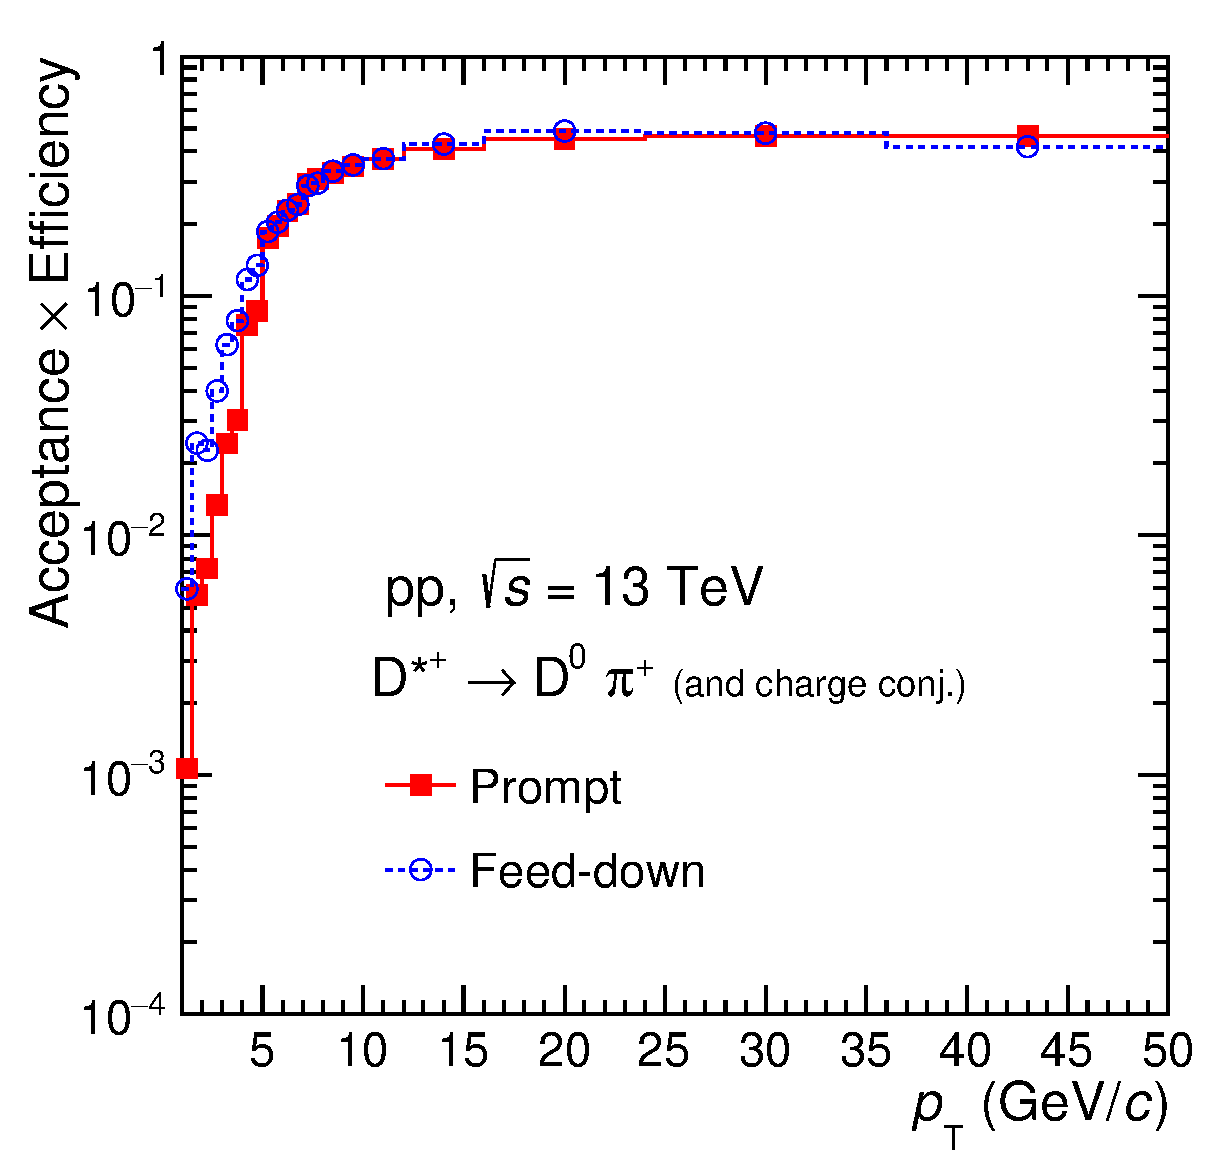
\includegraphics[width=0.8\textwidth]{figures/Dstar/pp13TeV/DstarAccEffVsPt_pp_13TeV.eps}
\caption{Transverse momentum dependence of efficiency$\times$acceptance for prompt (black) and feed-down (red).}
\label{fig:Dstar_eff}
\end{center}
\end{figure}
% Dplus efficiency

